\documentclass{amsart}

\usepackage{graphicx}

\hyphenation{ge-ne-ra-tors}

\title[SCSCP Specification]{Symbolic Computation Software Composability Protocol (SCSCP) specification \\ Version 1.3}

\author{S.~Freundt, P.~Horn, A.~Konovalov, S.~Linton, D.~Roozemond}

\address{Sebastian Freundt
\newline Fakult\"at II - Institut f\"ur Mathematik, 
\newline Technische Universit\"at Berlin, Berlin, Germany}
\email{freundt@math.tu-berlin.de}

\address{Peter Horn
\newline Fachbereich Mathematik, Universit\"at Kassel, Kassel, Germany}
\email{hornp@mathematik.uni-kassel.de} 

\address{Alexander Konovalov
\newline School of Computer Science, University of St Andrews,
\newline North Haugh, St Andrews, Fife, KY16 9SX, Scotland}
\email{alexk@cs.st-and.ac.uk}

\address{Steve Linton
\newline School of Computer Science, University of St Andrews, 
\newline North Haugh, St Andrews, Fife, KY16 9SX, Scotland}
\email{sal@cs.st-and.ac.uk}

\address{Dan Roozemond
\newline Department of Mathematics and Computer Science,
\newline Technische Universiteit Eindhoven, 
\newline HG 9.55, Postbus 513, 5600 MB Eindhoven, Netherlands}
\email{d.a.roozemond@tue.nl} 

\thanks{The project 026133 ``SCIEnce - Symbolic Computation Infrastructure in Europe'' is supported by the EU FP6 Programme}

\begin{document}

\thispagestyle{empty}
\hspace{-15mm}
\begin{minipage}{60mm}
	\rule{0pt}{0pt}\par\vfill
	
\includegraphics[width=60mm]{SCSCP_logo}
	\par\vfill\rule{0pt}{0pt}
\end{minipage} 
\ \hspace{50mm} 
\begin{minipage}{40mm}
	\rule{0pt}{0pt}\par\vfill
	
\includegraphics[width=40mm]{SCIEnce_logo}
	\par\vfill\rule{0pt}{0pt}
\end{minipage} 

\vspace{15mm}

\begin{center}
\sc
\Large
S. Freundt,
P. Horn,
A. Konovalov, \\
S. Linton,
D. Roozemond \\
\vspace{10mm}
\Huge 
Symbolic Computation Software Composability Protocol \\
\vspace{10mm}
SCSCP\\
\vspace{10mm}
Specification, 
Version 1.3 \\
\vspace{10mm}
\Large
\today \\
\vspace{40mm}
{\Small The project 026133 ``SCIEnce - Symbolic Computation Infrastructure in Europe'' \\
is supported by the EU FP6 Programme}
\end{center}

\newpage

\tableofcontents
\newpage

%#########################################
\section{Introduction}
%#########################################

This document specifies the requirements for the software to be developed
by the NA3 activity of the SCIEnce project for the subsequent usage in the
NA3 and JRA1 activities.

Specifically it describes a protocol by which a CAS may offer
services and a client may employ them. This protocol is called the
{\it Symbolic Computation Software Composability Protocol}, or {\bf SCSCP}.
We envisage clients for this protocol including:

\begin{itemize}
\item A Web server which passes on the same services as Web services
  using SOAP/HTTP to a variety of possible clients;
\item Grid middleware;
\item Another instance of the same CAS (in a parallel computing context);
\item Another CAS running on the same system.
\end{itemize}

Note that the specification assumes two possible ways of implementation.
One is the standard socket-based implementation, where a CAS can 
talk locally or remotely via ports, as described in the section \ref{implement},
in fact an SCSCP service rather than a Web service. 
The other implementation is a proper Web service using standard SOAP/HTTP wrappings for SCSCP messages. 
In the SCSCP specification we will use the term {\it Web services} in the broad sense, 
meaning both kinds of symbolic computation services.

Our vision of the SCSCP usage is described in the following scheme.

\centerline{\resizebox{130mm}{!}{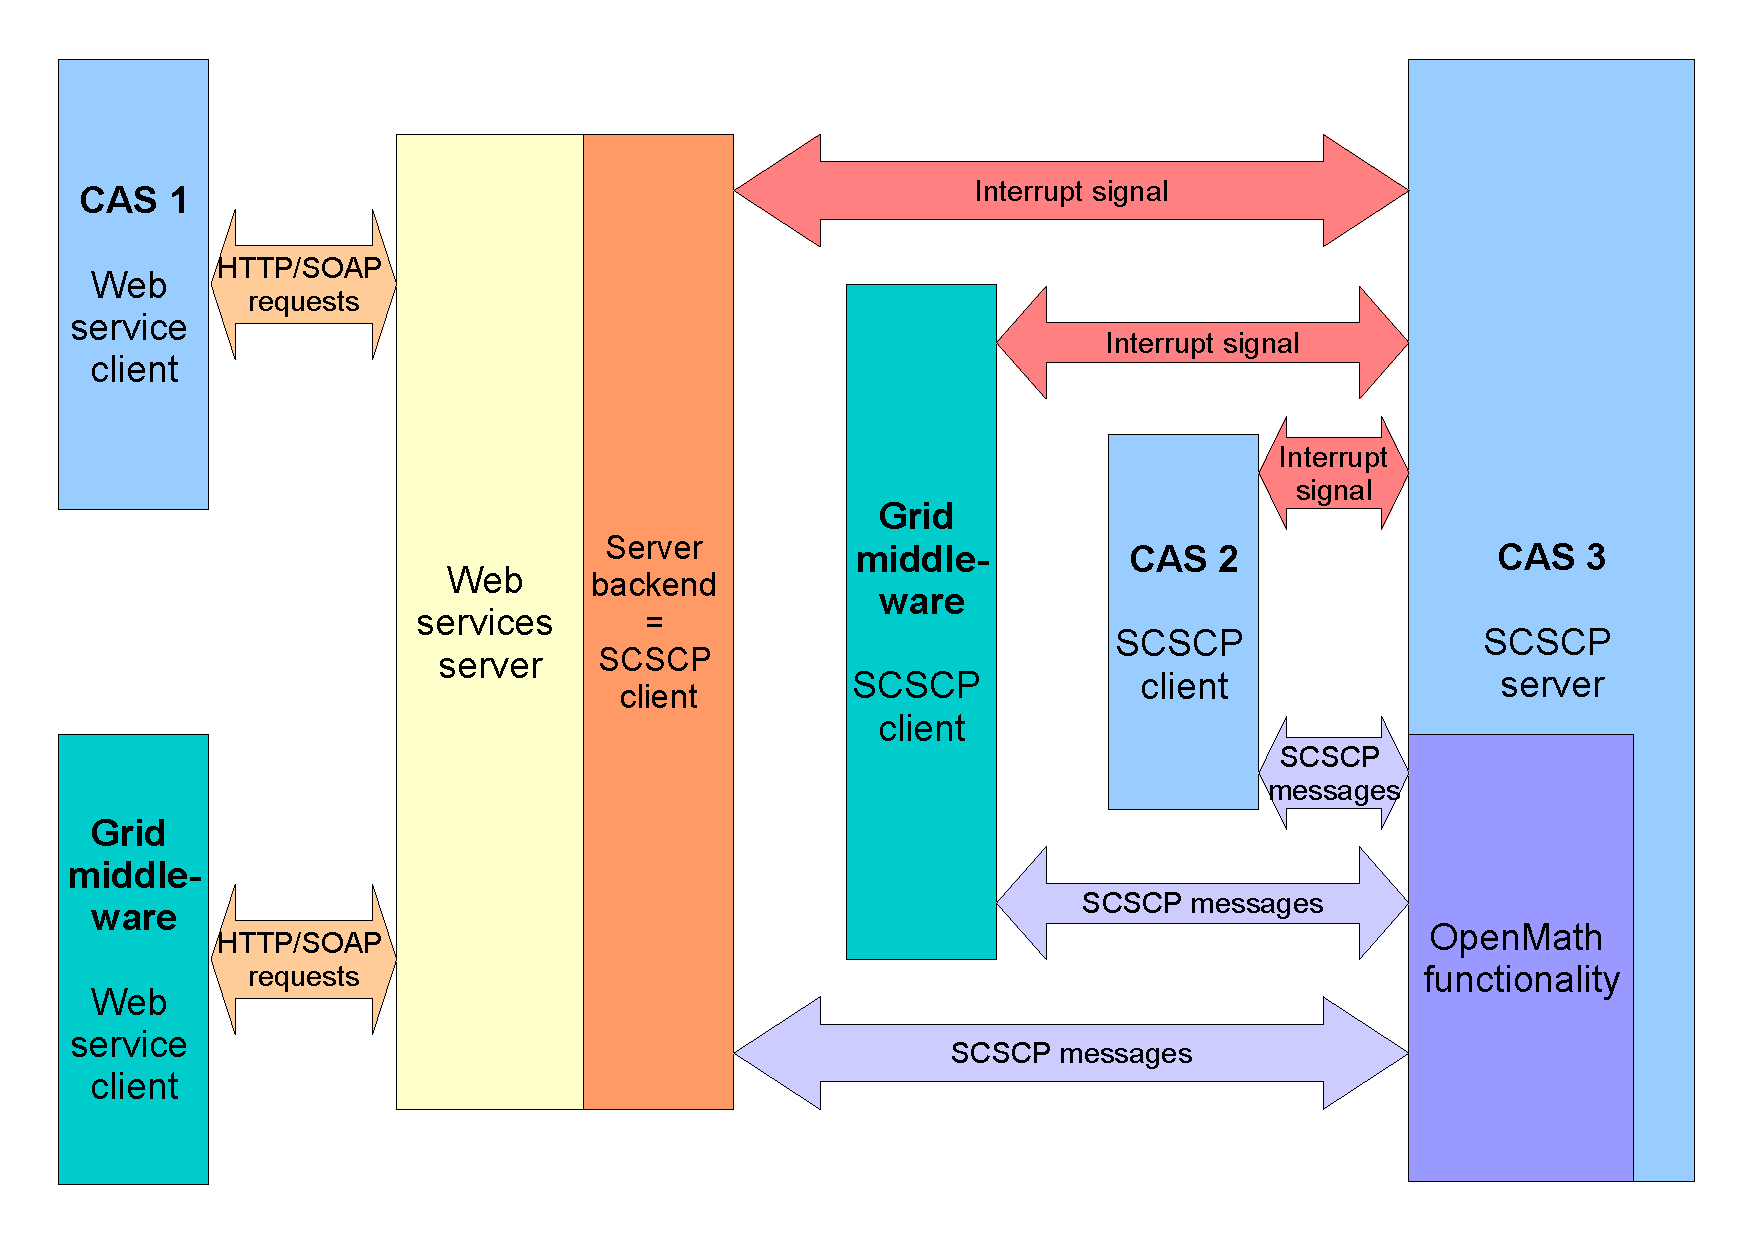
\includegraphics{scheme_SCSCP}}}

\centerline{\small{Figure 1. SCSCP usage.}}
\vspace{15pt}

In Section \ref{semantic} we describe the meaning of the possible messages
that can appear during communication between various software and the
allowed sequences of such messages. In Section \ref{tech} we
specify how these messages are encoded as OpenMath objects. 
Finally in Section \ref{implement} we describe one
solution (suitable for UNIX systems, at least) for the practical
problems of establishing a connection and delivering these messages.

In Appendix A we specify the list of necessary OpenMath symbols.
Examples of OpenMath messages are given in Appendices B and C.  
More examples may be found in the {\tt scscp1} and {\tt scscp2} OpenMath 
Content Dictionaries: \cite{scscp1}, \cite{scscp2}.
\vspace{5pt}

List of abbreviations used in the document:
\begin{description}
\item[CAS] Computer Algebra System
\item[CD] Content Dictionary 
\item[OM] OpenMath 
\item[PI] processing instruction (in XML)
\item[SCSCP] Symbolic Computation Software Composability Protocol 
\item[WS] Web Service 
\item[WSDL] Web Services Description Language 
\end{description}


%#########################################
\section{Semantic descriptions}\label{semantic}
%#########################################
 
\subsection{Messages from client to server}

\subsubsection{Procedure call}\label{sec_semantic_msgs_procedurecall}

This is an OM message containing the following information:
\begin{itemize}
\item {\it Procedure name} - the name of the procedure registered as a web-service;
\item {\it Arguments} - arguments that will be passed to the procedure being called;
      (Remark: we treat procedure options, such as guidance options for used algorithms, as
      arguments as well);
\item {\it Options/Attributes} - attributes and options that specify the expected behaviour 
      of the system. Mandatory options are:
\begin{itemize}
    \item call identifier (unique in the scscp session);
    \item type of action performed with the result (precisely one must be given)
	\begin{itemize}
		\item storing the result at the server side and returning a cookie referring to it;
		\item returning the result of the procedure (that may involve the actual computation or the retrieval of a previously stored result);
		\item not returning the result itself, only a message indicating whether the procedure completed successfully or not;
	\end{itemize}
\end{itemize}
Non-mandatory options are, for example:
\begin{itemize}
	\item procedure runtime limit;
	\item minimal/maximal memory limits;
	\item debugging level, determining degree of output detail;
	\item other options that might appear during the development; may be system dependent.
\end{itemize}
\end{itemize}

There are some standard procedures predefined in Section \ref{spec-proc}. 
Besides this, in order to provide specific SCSCP services, the service provider should 
develop and make available their own customized procedures, which may range from 
generic services (e.g. we may imagine some procedure named like {\sf EVALUATE\_OMOBJ} 
to evaluate given OM object) to specific (e.g. compute the determinant of a matrix).

\subsubsection{Interrupt signal}
This signal implies that the results of one particular computation are not needed, so the CAS need not complete the computation. After receiving an interrupt signal, the server must, as always, reply to the procedure call with the mentioned call ID. It must still reply to the procedure calls in the order they were received in. For example, if the client sends procedure calls $A$,$B$,$C$ and then an interrupt signal for $B$ while the server is still computing $A$, the server must still reply to $A$ before it sends a procedure terminated message for $B$.

Note that it is always correct for a CAS to ignore an interrupt, and thus simply reply with a procedure completed message. This may be appropriate when procedure calls are quick.

Note also that in earlier versions of the protocol the Interrupt signal was implemented using POSIX signals, but from version 1.3 onwards the signal is implemented by the {\tt <?scscp terminate?>} processing instruction. See Section \ref{sec_impl_interrupt}.

\subsection{Messages from server to client}

\subsubsection{Procedure completed}

This is an OM message containing the information about the result of the procedure:
\begin{itemize}
\item {\it Result value} - if the procedure returns a result, it must be contained in 
this section of the message. 
If the procedure only produces side-effects, such a section is not necessary since
this message itself acts as a signal about its successful completion;
\item {\it Mandatory additional information:}
\begin{itemize}
\item call identifier;
\end{itemize}
\item {\it Optional additional information:}
\begin{itemize}
\item procedure runtime;
\item memory used;
\item other information that we might need (may be system dependent).
\end{itemize}
\end{itemize}

\subsubsection{Procedure terminated}

This is an OM message that acts as a signal about procedure termination.
\begin{itemize}
\item {\it Error}\,: in its body, the message must contain an appropriate error, as described for example in the {\tt scscp1} OpenMath Content Dictionary.
\item {\it Mandatory additional information:}
\begin{itemize}
\item call identifier;
\end{itemize}
\item {\it Optional additional information:}
\begin{itemize}
\item procedure runtime before termination;
\item memory used;
\item other information that we might need (may be system dependent).
\end{itemize}
\end{itemize}

\subsection{Allowed sequences of messages}\label{sec_semt_allowedseq}

Once a connection has been established and any initial technical
information exchanged (the mechanism for which is
part of an implementation of this protocol and addressed in Section
\ref{implement}) the SCSCP session is considered to be opened.

Until the end of the session, the communication from client to server is 
a stream of procedure calls and the response is a stream of procedure 
completed and/or procedure terminated messages. The client is permitted 
to send as many procedure calls as it likes, subject to the buffering 
capabilities of the channel used in a particular implementation. The server must
process them in sequence and send {\it either} a procedure completed, 
{\it or} a procedure terminated message (but not both) for each procedure call received.

Apart from this, the client can send an interrupt message to the server.
The interrupt message can be sent to the server at any time. 
It entitles the server to stop processing one procedure call and 
respond to it with a suitable procedure terminated message. 

\section{Special Procedures}\label{spec-proc}

This section documents certain predefined procedures which every
compliant client is expected to support. OpenMath symbols corresponding
to these procedures are defined in the \verb|scscp2| Content
Dictionary \cite{scscp2}.

\subsection{Determining the list of supported procedures}

\subsubsection {Representing Collections of OpenMath Symbols}

A number of the procedures defined in this section return values which
are intended to represent sets of OM symbols. For convenience, we
define a standard way of representing these sets. 

Such sets should be represented as applications of the symbol
\verb|symbol_set| which may take any number of arguments. Each of those
arguments should be one of the following:

\begin{enumerate}
\item An OpenMath symbol, representing itself,
\item An application of one of symbols \verb|CDName| or \verb|CDURL|
      from the \verb|meta| CD, representing all the symbols in the referenced CD;
\item An application of one of the symbols \verb|CDGroupName| or
      \verb|CDGroupURL| from the \verb|metagrp| CD;
      representing all the symbols in all CDs in the referenced CD group.
\end{enumerate}

As an alternative, the symbol \verb|symbol_set_all| can be used, to
represent the set of all OpenMath symbols from any CD.

\subsubsection {Transient CDs}\label{sec_special_transient}

In describing its allowed procedure calls according to the conventions
of this section, a server is permitted to refer to symbols from CDs with
names beginning \verb|scscp_transient_| (note the lower case). 
These are content dictionaries
defined by this server, and valid only for the duration of the
session. If needed, the client can request these CDs using the
\verb|get_transient_cd| procedure (see below).

\subsubsection{Requesting the Allowed Procedure Names}

The first standard procedure defined in this section is
\verb|get_allowed_heads|, which takes no arguments. 
This returns, in the above format, the set of
OpenMath symbols which might be allowed to appear as ``head'' symbol (ie
first child of the outermost \verb|<OMA>|) in an SCSCP procedure call to
this server. These may be symbols from standard OpenMath CDs or from
transient CDs as described above. 

A second standard procedure is \verb|is_allowed_head|. It takes only one
argument, which is to be an OpenMath symbol. The server returns a boolean,
\verb|logic1.true| or \verb|logic1.false|, depending on whether it accepts this
symbol. This enables the client to check whether a particular symbol is allowed
without requesting the full symbol list.

Note that it is acceptable (although
not necessarily desirable) for a server to
``overstate'' the set of symbols it accepts and use standard OpenMath
errors to reject requests later.

\subsubsection{Requesting Signature Information}

The standard procedure \verb|get_signature| takes one argument: an
OpenMath symbol. If the supplied symbol is one of those accepted as a
head symbol by the server then it returns an application of the \verb|signature|
symbol. This symbol takes four arguments: 
\begin{itemize}
\item an OpenMath symbol indicating which signature is described; 
\item a minimum number of children ({\it min}); 
\item a maximum number of children ({\it max}), 
      which could be the \verb|infinity| symbol from the \verb|nums1| CD); 
\item a set of symbols, represented as an application of the
      symbol \verb|symbol_set|, or a list of \verb|symbol_set|s:
\begin{itemize}
\item if the list of \verb|symbol_set|s is given, then its $i$-th entry
      corresponds to the $i$-th argument;
\item if just one \verb|symbol_set| is given, it represents that every argument
      should come from this set.
\end{itemize}
\end{itemize}


\subsubsection{Requesting Transient CDs}

The standard procedure \verb|get_transient_cd| takes one argument -- an
application of the \verb|CDName| symbol from \verb|meta|, which should
start with \verb|scscp_transient_|, and returns the corresponding CD, encoded
using symbols from the \verb|meta| CD.  If no such transient CD is
defined by this server it returns the \verb|procedure_terminated| message
with OM error containing the symbol \verb|no_such_transient_cd| 
(from the \verb|scscp2| CD) and the name of the CD that caused the problem. 

\subsubsection{Requesting general description of the service}

The service provider may have various parameters describing an offered service.
The connection initiation message contains only the service name, version and 
identifier, and this is not enough. Instead of this, some meta-information
about the service may be structured and retrieved by a special standard
procedure \verb|get_service_description|. It takes no arguments, since it is
completely determined by the server to which it was sent, and returns the
symbol \verb|service_description| that takes the following three arguments as OM strings:
server name, version and the description of the service. The latter may include
for example functions exposed, resources, contact details of service provider, etc.
%\footnote{should we specify more precisely what must be in the description
%or provide a template for it? I (AK) think the description may be a list
%of pairs "field\_name" - "string description", and the template may have
%some recommended set of field names. Then I can convert them into a GAP
%record, for example)}

\subsection{Operations with remote objects}

\subsubsection{Storing, retrieving and deleting remote objects}

The following symbols are defined in the \verb|scscp2| CD \cite{scscp2} 
to work with remote objects:
\begin{description}
\item[\tt{store\_session}] store an object on the server side (possibly
after computing or simplyfying it), 
returning a cookie (actually, an OM reference) pointing to that object.
This cookie is then usable within the current session to get access
to the actual object;
\item[\tt{store\_persistent}] store an object on the server side (possibly
after computing or simplyfying it), 
returning a cookie (actually, an OM reference) pointing to that object.
This cookie is then usable in the foreseeable future, possibly from 
different sessions, to get access to the actual object;
\item[\tt{retrieve}] using the cookie that was obtained earlier by 
one of the store procedures or another procedure call, return 
an OM object representing the object referred by the cookie; 
\item[\tt{unbind}] remove the object referred by the cookie from the server. 
\end{description}
The service provider should be able to decide whether clients are
allowed to create remote objects or not.

%#########################################
\section{Technical descriptions}\label{tech}
%#########################################

\subsection{Messages from client to server}

\subsubsection{Procedure call}

The procedure call is an OM object having in general
the following structure:

\begin{verbatim}
<OMOBJ>
    <OMATTR>
        <!-- call_id and option_return_... are mandatory -->
        <OMATP>
            <OMS cd="scscp1" name="call_id" />
            <OMSTR>call_identifier</OMSTR>
            <OMS cd="scscp1" name="option_runtime" />
            <OMI>runtime_limit_in_milliseconds</OMI>
            <OMS cd="scscp1" name="option_min_memory" />
            <OMI>minimal_memory_required_in_bytes</OMI>
            <OMS cd="scscp1" name="option_max_memory" />
            <OMI>memory_limit_in_bytes</OMI>
            <OMS cd="scscp1" name="option_debuglevel" />
            <OMI>debuglevel_value</OMI>
            <OMS cd="scscp1" name="option_return_object" />
            <OMSTR></OMSTR>
        </OMATP>
        <!-- Attribution pairs finished, now the procedure call -->
        <OMA>
            <OMS cd="scscp1" name="procedure_call" />
            <OMA>
                <OMS cd="..." name="..."/> 
                <!-- Argument 1 -->
                <!-- ... -->
                <!-- Argument M -->
            </OMA>
        </OMA>
    </OMATTR>
</OMOBJ>
\end{verbatim}

Remarks:
\begin{enumerate}
\item
The first OM object in the argument of \verb|procedure_call| is the 
name of the procedure, the remaining OM objects are its arguments. It may come
from any (standard or non-standard) content dictionary, including transient CDs
such as described in Section \ref{sec_special_transient}. 
\item
OM symbols for options will be introduced accordingly to the list of options
given in Section \ref{sec_semantic_msgs_procedurecall}. 
If the need for new options is discovered, new OM
symbols for them will be added to future CDs.
\item
Options (except the \verb|call_id| and one of the options \verb|option_return_cookie|, \\
\verb|option_return_nothing| or \verb|option_return_object|) 
may be omitted in the procedure call, 
and in this case their default values must be used.
The default values of options may be determined by
the service provider, and they are not regulated by the
SCSCP specification.
\end{enumerate}

\subsubsection{Interrupt signal}

See Section \ref{sec_impl_interrupt}.

\subsection{Messages from server to client}

\subsubsection{Procedure completed}

The procedure completion message is an OM object having in general 
the following structure:

\begin{verbatim}
<OMOBJ>
    <OMATTR>
        <!-- Attribution pairs (only call_id is mandatory) -->
        <OMATP>
            <OMS cd="scscp1" name="call_id" />
            <OMSTR>call_identifier</OMSTR>
            <OMS cd="scscp1" name="info_runtime" />
            <OMI>runtime_in_milliseconds</OMI>
            <OMS cd="scscp1" name="info_memory" />
            <OMI>used_memory_in_bytes</OMI>
            <OMS cd="scscp1" name="info_message" />
            <OMSTR>some extra information</OMSTR>
        </OMATP>    
        <!-- Attribution pairs finished, now the result -->
        <OMA>
            <OMS cd="scscp1" name="procedure_completed" />
            <!-- The result itself, may be OM symbol for cookie -->
            <!-- OM_object_corresponding_to_the_result -->
        </OMA>
    </OMATTR>
</OMOBJ>
\end{verbatim}


In case the procedure returns a cookie, the returned OM object must
have the following structure:

\begin{verbatim}
<OMOBJ>
    <OMATTR>
        <OMATP>
            <OMS cd="scscp1" name="call_id" />
            <OMSTR>call_identifier</OMSTR>
        </OMATP>
        <OMA> 
            <OMS cd="scscp1" name="procedure_completed" />
            <OMR href="CAS_variable_identifier" />
        </OMA>
    </OMATTR>
</OMOBJ>
\end{verbatim}

\subsubsection{Procedure terminated}

The procedure termination message is an OM object having 
in the most general case the following structure:

\begin{verbatim}
<OMOBJ>
    <OMATTR>
       <!-- Attribution pairs (only call_id is mandatory) -->
        <OMATP>
            <OMS cd="scscp1" name="call_id" />
            <OMSTR>call_identifier</OMSTR>
            <OMS cd="scscp1" name="info_runtime" />
            <OMI>runtime_in_milliseconds</OMI>
            <OMS cd="scscp1" name="info_memory" />
            <OMI>used_memory_in_bytes</OMI>
        </OMATP> 
        <!-- Attribution pairs finished, now the error message -->
        <OMA>
            <OMS cd="scscp1" name="procedure_terminated" />
            <OME>
                 <OMS cd="scscp1" name="name_of_standard_error"/>
                 <!-- Error description depends on error type -->
                 <OMSTR>Error_message</OMSTR>
            </OME>
        </OMA>
    </OMATTR>
</OMOBJ>
\end{verbatim}

%#########################################
\section{Reference Implementation}\label{implement}
%#########################################

In this section we describe a simple implementation.

To facilitate the implementation, we use XML processing instructions (PI). 
All PIs defined by SCSCP specification have the form
\begin{verbatim}
<?scscp [key] [attribute="value" [attribute="value" [...]]] ?>
\end{verbatim}
where:
\begin{itemize}
\item {\tt key} is an alphanumerical identifier,
\item {\tt attribute} is an alphanumerical identifier,
\item {\tt value} is an arbitrary string with the same constraints as an XML URI,
unless stated otherwise.
\end{itemize}
A single SCSCP processing instruction must not exceed 4094 bytes 
in total, including \verb|<?| and \verb|?>| elements. 
Furthermore, any processing instruction with an unrecognized key must be ignored.

\subsection{Connection Initiation}

The software wishing to provide an SCSCP service should listen on port 26133.
This port has been assigned to SCSCP by the Internet Assigned Numbers Authority 
(IANA) in November 2007, see \\ \verb|http://www.iana.org/assignments/port-numbers|. 

If the port is already in use, for example in a parallel computing context, the SCSCP
service may listen on another port, for example by increasing the port number by one
until an available port is found.

When a client connects, the server should send it a Connection Initiation
Message, agree about the protocol version, and then commence an
exchange of messages as desribed in Section \ref{sec_semt_allowedseq}.

\subsubsection{Connection Initiation Message}

This processing instruction is the first message that the client 
receives from the server in the beginning of the SCSCP session.
Is has the following format:
\begin{verbatim}
<?scscp service_name="name" service_version="ver" 
  service_id="id" scscp_versions="list_of_supported_versions" ?> 
\end{verbatim}
where
\begin{itemize}
\item {\tt "name"} is a string containing the service name, 
e.g. {\tt "GAPSmallGroups"}, {\tt "KANT"},  {\tt "MapleIntegration"}, {\tt "MuPAD"}, etc.
\item {\tt "ver"} is a string containing the version of the service, 
e.g. {\tt "11"}, {\tt "3.1"}, {\tt "4.1.5beta"}, etc.
\item {\tt "id"} is an identifier for the service, {\bf unique} within
the SCSCP session (e.g. a hostname-pid combination, a pid, etc.).
Note that when the hostname is used, it is advised not to trim off any domain 
information from the hostname to avoid situations when the client connected 
to multiple hosts may get coinciding service identifiers.
\item \verb|scscp_versions| is a space-separated list of identifiers of
SCSCP versions supported by the server. Identifier of every single 
version of SCSCP may contain digits, letters and dots. 
Versions can be listed in any order.
For example, valid value of \verb|scscp_versions| is
\verb|"1.0 3.4.1 1.2special"|.
\end{itemize}
The format of the control sequence is compulsory, and server implementations 
must not change the order of the attribute/value pairs nor omit some of them. 
This strict restriction makes it sure that even very simple clients should be 
able to parse this control sequence.

After receiving an incoming connection from a client, the SCSCP server must not 
send to the client anything else before the connection initiation message. 
The client must wait for this "welcome string" from the server, and must 
not send any data to the server before obtaining it.

\subsubsection{Version negotiation}

To ensure compatibility of various versions of the protocol both upwards and 
downwards the following version negotiation procedure
should be performed.

After obtaining the connection initiation message from the server,
the client informs the server about the version of the protocol 
used by the client, sending the message
\begin{verbatim}
<?scscp version="client_version" ?>
\end{verbatim}
where \verb|"client_version"| is a string denoting the
SCSCP versions supported by the client (for example, 
{\tt "1.0"} or {\tt "3.4.1"} or {\tt "1.2special"}). 

As the current rule, we require that an official SCSCP client/server 
should always support at least the version {\tt "1.0"}. 

We expect that the client choose one of the versions listed in the
connection initiation message received from the server. However,
a simple client may ignore that information, because
the server is able to reject any incompatible versions the client may propose.
After receiving the client's SCSCP versions, the server replies with one of two 
possible messages:
\begin{itemize}
\item \verb|<?scscp quit reason="not supported version" ?>|,
if the server does not support the version communicated by the client. 
The server should subsequently close the connection.
\item \verb|<?scscp version="server_version" ?>| if the server does
support the version communicated by the client. Here \verb|"server_version"| 
is a string representing the preferred SCSCP version of the server. 
The server should subsequently wait for messages from the client.
\end{itemize}

Remember that in the connection initiation phase, the order of messages is very strict:
\begin{itemize}
\item after receiving an incoming connection, the SCSCP server must not 
send anything to the client before the Connection Initiation Message,
\item the client must wait for the Connection Initiation Message from the server, 
and must not send any data to the server before obtaining this message,
\item after receiving the Connection Initiation Message the client must send
its version to the server,
\item after receiving the client's version, the server either confirms this
to the client and starts to wait for procedure calls, or rejects it by replying
with the quit message,
\item only after receiving the server's confirmation of the protocol version, 
the client is allowed to send procedure calls to the server.
\end{itemize}
Any other data sent in this phase may be ignored.

The only other allowed control sequence during this phase of the protocol 
is {\tt <?scscp quit ?>} or \verb|<?scscp quit reason="explanation" ?>|, 
issued, for example, when one side is not able to 
accept any version proposed by the other side, or issued under external 
circumstances, for example, sending messages that are not allowed in this
negotiation phase. In either case, the rules of quitting (see below) are applied.

An example of successful version negotiation:
\begin{verbatim}
Server -> Client:
  <?scscp service_name="MuPADserver" service_version="1.1" 
    service_id="host:26133" scscp_versions="1.0 3.4.1 1.2special" ?>
Client -> Server: 
  <?scscp version="1.0" ?>
Server -> Client: 
  <?scscp version="1.0" ?>
\end{verbatim}

An example of failed version negotiation:
\begin{verbatim}
Server -> Client:
  <?scscp service_name="MuPADserver" service_version="1.1" 
    service_id="host:26133" scscp_versions="1.0 3.4.1 1.2special" ?>
Client -> Server: 
  <?scscp version="1.5beta" ?>
Server -> Client: 
  <?scscp quit reason="non supported version 1.5beta" ?>
\end{verbatim}

\subsection{Ongoing message exchange}

All messages except interrupts are delivered as XML processing instructions and
OpenMath objects in either the XML or the binary OpenMath encoding, transmitted 
via the socket connection.

To locate OpenMath objects in the input/output streams, we put them into
{\it transaction blocks}. The transaction block looks as follows:
\begin{verbatim}
<?scscp start ?>
[a valid OpenMath object]
<?scscp end ?>
\end{verbatim}
Another kind of transaction block have the form 
\begin{verbatim}
<?scscp start ?>
[something]
<?scscp cancel ?>
\end{verbatim}
and the {\tt <?scscp cancel ?>} instruction indicates that
the started transaction block is cancelled. The receiver need not to
wait for a matching {\tt <?scscp end ?>} directive, and must not 
process/evaluate the data in this transaction block. 

Another instruction is {\tt <?scscp quit ?>}, which may also be 
used in the long form \verb|<?scscp quit reason="explanation" ?>|,
that indicates that the 
sender is about to leave the SCSCP session. Then each side may close
the socket (and at least the receiver may safely disconnect). This 
instruction may appear anywhere throughout the session.

Any data after successful version negotiation which are located
outside of transaction blocks (apart from PIs) may be safely ignored. 

\subsection{Interrupt}\label{sec_impl_interrupt}
The client may send a processing instruction carrying an
interrupt signal as follows:
\begin{verbatim}
<?scscp terminate call_id="someidentifier" ?>
\end{verbatim}
This PI implies that the results of the computation with call ID \verb|someidentifier|
are not needed, so the server need not complete the computation.
The server may still choose to complete the calculation.

The server must, as always, reply to the \verb|procedure_call| with the mentioned
call ID. It may do this either by sending a \verb|procedure_terminated| or, if the
result is already available, a \verb|procedure_completed| message.

Note that it is always correct for a server to ignore an interrupt, and
that this may be appropriate when procedure calls are quick.

\subsection{Info messages}
We finally describe PIs carrying some information that is not critical for the
functioning of the protocol. These PIs have the form
\begin{verbatim}
<?scscp info="some interesting information" ?>
\end{verbatim}
and may be sent by both the client and the server. They may aid in 
debugging a protocol implementation.

\subsection{Other ways of implementation}
We assume that in most cases it will be enough for the SCSCP-compliant
server to support the scheme outlined above, since this provides the
opportunity to ``talk'' in clean SCSCP with other servers supporting this
scheme.
It also allows communication with the SCSCP-proxy server, that accepts
SOAP/HTTP requests from the outside and then sends their SCSCP 
content to servers. 
However, it is not unconceivable that the server itself is able to receive
SOAP/HTTP requests without the mentioned proxy. 

The same refers to the client functionality: if there is a server
that accepts only SOAP/HTTP requests, then this server can send an SCSCP-request 
to the proxy which will then act as a proper Web services client, or might 
be able to wrap an SCSCP procedure call into a SOAP/HTTP envelope itself. 

\newpage

\appendix
\section{The {\tt scscp1} and {\tt scscp2} OM CDs}

\vspace{5pt}

\centerline{ \bf {The list of OM symbols defined in the {\tt scscp1} CD}}

\vspace{10pt}

The {\tt scscp1} CD \cite{scscp1} defines OM symbols 
for main types of messages and attributes that may appear in them:

\begin{enumerate}
\item Main messages:
\begin{itemize}
\item \verb|procedure_call|
\item \verb|procedure_completed|
\item \verb|procedure_terminated|
\end{itemize}
\item Call and response identifiers:
\begin{itemize}
\item \verb|call_id|
\end{itemize}
\item Options in procedure calls:
\begin{itemize}
\item \verb|option_max_memory|
\item \verb|option_min_memory|
\item \verb|option_runtime|
\item \verb|option_debuglevel|
\item \verb|option_return_cookie|
\item \verb|option_return_object| 
\item \verb|option_return_nothing| 
\end{itemize}
\item Information attributes:
\begin{itemize}
\item \verb|info_memory|
\item \verb|info_runtime|
\item \verb|info_message|
\end{itemize}
\item Standard errors:
\begin{itemize}
\item \verb|error_memory|
\item \verb|error_runtime|
\item \verb|error_system_specific|
\end{itemize}
\end{enumerate}

\noindent See the {\tt scscp1} CD \cite{scscp1} for the appropriate descriptions.

\newpage

\centerline{ \bf {The list of OM symbols defined in the {\tt scscp2} CD}}

\vspace{10pt}

The {\tt scscp2} CD \cite{scscp2} defines OM symbols for special procedures, and also
some symbols that may appear in their arguments and results:

\begin{enumerate}
\item Procedures for work with remote objects:
\begin{itemize}
\item \verb|store_session|
\item \verb|store_persistent|
\item \verb|retrieve|
\item \verb|unbind|
\end{itemize}
\item Special procedures to obtain meta-information about SCSCP service:
\begin{itemize}
\item \verb|get_allowed_heads|
\item \verb|is_allowed_head|
\item \verb|get_transient_cd|
\item \verb|get_signature|
\item \verb|get_service_description|
\end{itemize}
\item Special symbols:
\begin{itemize}
\item \verb|signature|
\item \verb|service_description|
\item \verb|symbol_set|
\item \verb|symbol_set_all|
\item \verb|no_such_transient_cd|
\end{itemize}
\end{enumerate}

\noindent See the {\tt scscp2} CD \cite{scscp2} for the appropriate descriptions.

\newpage

\section{Examples of OM messages}

\subsection{The Procedure Call message}

The \verb|GroupIdentificationService| procedure accepts a permutation group $G$
given by its generators and returns the \verb|procedure_completed|
message with the number of this group in the GAP Small Groups Library.
If this fails, for example because groups of order $|G|$ are
not contained in that library or because identification for groups of such order
is not available in GAP, it sends a \verb|procedure_terminated| message.

\begin{verbatim}
<OMOBJ>
    <OMATTR>
        <OMATP>
            <OMS cd="scscp1" name="call_id" />
            <OMSTR>symcomp.org:26133:18668:s2sYf1pg</OMSTR>
            <OMS cd="scscp1" name="option_runtime" />
            <OMI>300000</OMI>
            <OMS cd="scscp1" name="option_min_memory" />
            <OMI>40964</OMI>
            <OMS cd="scscp1" name="option_max_memory" />
            <OMI>134217728</OMI>
            <OMS cd="scscp1" name="option_debuglevel" />
            <OMI>2</OMI>
            <OMS cd="scscp1" name="option_return_object" />
            <OMSTR></OMSTR>
        </OMATP>
        <OMA>
            <OMS cd="scscp1" name="procedure_call" />
            <OMA>
                <OMS cd="scscp_transient_1" 
                   name="GroupIdentificationService" />
                <OMA>
                    <OMS cd="group1" name="group"/>
                    <OMA>
                        <OMS cd="permut1" name="permutation"/>
                        <OMI> 2</OMI> <OMI> 3</OMI>
                        <OMI> 1</OMI>
                    </OMA>
                    <OMA>
                        <OMS cd="permut1" name="permutation"/>
                        <OMI> 1</OMI> <OMI> 2</OMI>
                        <OMI> 4</OMI> <OMI> 3</OMI>
                    </OMA>
                </OMA>        
            </OMA>
        </OMA>
    </OMATTR>
</OMOBJ>

\end{verbatim}

In the next example we retrieve the group [24,12] from GAP Small Groups Library,
creating it on the GAP side and requesting a cookie for it:

\begin{verbatim}
<OMOBJ>
    <OMATTR>
        <OMATP>
            <OMS cd="scscp1" name="call_id" />
            <OMSTR>symcomp.org:26133:18668:GvnaGRLN</OMSTR>
            <OMS cd="scscp1" name="option_return_cookie" />
            <OMSTR></OMSTR>
        </OMATP>
        <OMA>
            <OMS cd="scscp1" name="procedure_call" />
            <OMA>
                <OMS cd="scscp_transient_1" name="GroupByIdNumber" />
                <OMI>24</OMI><!-- Arg1 -->
                <OMI>12</OMI><!-- Arg2 -->
            </OMA>    
        </OMA>
    </OMATTR>
</OMOBJ>
\end{verbatim}

In the next example we are sending an OM object containing a MathML object:

\begin{verbatim}
<OMOBJ>
  <OMATTR>
    <OMATP>
      <OMS cd="scscp1" name="call_id"/>
      <OMSTR>symcomp.org:26133:18668:mDkmEqh9</OMSTR>
      <OMS cd="scscp1" name="option_return_cookie"/>
      <OMSTR></OMSTR>
    </OMATP>
    <OMA><OMS cd="scscp1" name="procedure_call"/>
      <OMA>
        <OMS cd="scscp_transient_M25" name="Evaluate" />
        <OMA>
          <OMS cd="altenc" name="MathML_encoding"/>
          <OMFOREIGN encoding="MathML-Presentation">
            <math xmlns="http://www.w3.org/1998/Math/MathML">
              <mrow>
                <mi>sin</mi>
                <mo>&ApplyFunction;</mo>
                <mfenced><mi>x</mi></mfenced>
              </mrow>
            </math>
          </OMFOREIGN>
        </OMA>
      </OMA>
    </OMA>
  </OMATTR>
</OMOBJ>
\end{verbatim}

\newpage

\subsection{The Procedure Completed message}
The {\tt GroupIdentificationService} procedure from the previous example
returns its successful output in the following form:

\begin{verbatim}
<OMOBJ>
    <OMATTR>
        <OMATP>
            <OMS cd="scscp1" name="call_id" />
            <OMSTR>symcomp.org:26133:18668:s2sYf1pg</OMSTR>
            <OMS cd="scscp1" name="info_runtime" />
            <!-- The runtime in milliseconds as OM integer -->
            <OMI>1234</OMI>
            <OMS cd="scscp1" name="info_memory" />
            <!-- Memory occupied by CAS in bytes as OM integer -->
            <OMI>134217728</OMI>
        </OMATP>        
        <OMA>
            <OMS cd="scscp1" name="procedure_completed" />
            <OMA>
                <OMS cd="linalg2" name="vector"/>
                <OMI> 24</OMI>
                <OMI> 12</OMI>
            </OMA>
        </OMA>
    </OMATTR>
</OMOBJ>
\end{verbatim}

In case a cookie is requested, the 
\verb|procedure_completed| message may look as follows
(we assume the minimal debugging level with no information 
about the runtime and memory used):

\begin{verbatim}
<OMOBJ>
    <OMATTR>
        <OMATP>
            <OMS cd="scscp1" name="call_id" />
            <OMSTR>symcomp.org:26133:18668:GvnaGRLN</OMSTR>
        </OMATP>
        <OMA> 
            <OMS cd="scscp1" name="procedure_completed" />
            <OMR href="scscp://somehost.somedomain:26133/q9t4eX" />
        </OMA>
    </OMATTR>
</OMOBJ>
\end{verbatim}

\newpage

\subsection{The Procedure Terminated message}

This is an example how the server
may return an error message if the error arises at the CAS level
(we assume the minimal debugging level with no information 
about the runtime and memory used):

\begin{verbatim}
<OMOBJ>
    <OMATTR>
        <OMATP>
            <OMS cd="scscp1" name="call_id" />
            <OMSTR>symcomp.org:26133:18668:f1dG4fcT</OMSTR>
        </OMATP>
        <OMA>
            <OMS cd="scscp1" name="procedure_terminated" />
            <OME>
                 <OMS cd="scscp1" name="error_system_specific"/>
                 <OMSTR>Number of arguments must be 2</OMSTR>
            </OME>
        </OMA>
    </OMATTR>
</OMOBJ>
\end{verbatim}

\vspace{10pt}
One of standard errors on the SCSCP level may look as follows:
\vspace{5pt}

\begin{verbatim}
<OMOBJ>
    <OMATTR>
        <OMATP>
            <OMS cd="scscp1" name="call_id" />
            <OMSTR>symcomp.org:26133:18668:Sf3Rc6cT</OMSTR>
        </OMATP>
        <OMA>
            <OMS cd="scscp1" name="procedure_terminated" />
            <OME>
                 <OMS cd="scscp1" name="error_memory"/>
                 <OMSTR>Exceeded the permitted memory</OMSTR>
            </OME>
        </OMA>
    </OMATTR>
</OMOBJ>
\end{verbatim}

\newpage

\section{Examples of special procedures}

\subsection{List of supported procedures}

To find the list of procedures supported by the SCSCP server,
the client sends to the server the following message:

\begin{verbatim}
<OMOBJ>
    <OMATTR>
        <OMATP>
            <OMS cd="scscp1" name="call_id" />
            <OMSTR>symcomp.org:26133:18668:sRe6Gwqk</OMSTR>
            <OMS cd="scscp1" name="option_return_object" />
            <OMSTR></OMSTR>
        </OMATP>
        <OMA>
            <OMS cd="scscp1" name="procedure_call" />
            <OMA>
                <OMS cd="scscp2" name="get_allowed_heads" />
            </OMA>    
        </OMA>
    </OMATTR>
</OMOBJ>
\end{verbatim}

The server replies with the next message, demonstrating
all possible arguments of the \verb|symbol_set| OpenMath symbol:
symbols from transient CD, created by the service provider,
a symbol from a standard CD, a CD and a CD group.

\begin{verbatim}
<OMOBJ>
    <OMATTR>
        <OMATP>
            <OMS cd="scscp1" name="call_id" />
            <OMSTR>symcomp.org:26133:18668:KdeT54cV</OMSTR>
        </OMATP>        
        <OMA>
            <OMS cd="scscp1" name="procedure_completed" />
            <OMA>
                <OMS cd="scscp2" name="symbol_set"/>
                <OMS cd="scscp_transient_1" 
                   name="GroupIdentificationService" />
                <OMS cd="group1" name="group" />
                <OMA>
                    <OMS cd="meta" name="CDName"/>
                    <OMSTR>permut1</OMSTR>
                </OMA>  
                <OMA>
                    <OMS cd="metagrp" name="CDGroupName"/>
                    <OMSTR>scscp</OMSTR>
                </OMA>                         
            </OMA>
        </OMA>
    </OMATTR>
</OMOBJ>
\end{verbatim}

Now the client is interested in getting the transient CD \verb|scscp_transient_1|,
and sends to the server the procedure call displayed below.

Note that in this example we assume that the \verb|scscp_transient_1| 
CD contains just one symbol
{\tt GroupIdentificationService}, so the server could have just returned
{\tt CDName} with \verb|scscp_transient_1| as first argument instead of one symbol. 
In such a case the client may use \verb|get_transient_cd| procedure to get the
corresponding CD in order to find out which OM symbols are defined 
in it. 

\begin{verbatim}
<OMOBJ>
    <OMATTR>
        <OMATP>
            <OMS cd="scscp1" name="call_id" />
            <OMSTR>symcomp.org:26133:18668:aWeRvK2a</OMSTR>
            <OMS cd="scscp1" name="option_return_object" />
            <OMSTR></OMSTR>
        </OMATP>
        <OMA>
            <OMS cd="scscp1" name="procedure_call" />
            <OMA>
                <OMS cd="scscp2" name="get_transient_cd" />
                <OMA>
                    <OMS cd="meta" name="CDName"/>
                    <OMSTR>scscp_transient_1</OMSTR>
                </OMA>
            </OMA>        
        </OMA>
    </OMATTR>
</OMOBJ>
\end{verbatim}

In response to this procedure call, the server sends to the client 
the transient CD in the following message:

\begin{verbatim}
<OMOBJ>
    <OMATTR>
        <OMATP>
            <OMS cd="scscp1" name="call_id" />
            <OMSTR>symcomp.org:26133:18668:dLrHd64G</OMSTR>
        </OMATP>        
        <OMA>
            <OMS cd="scscp1" name="procedure_completed" />
            <OMA> 
                <OMS cd="meta" name="CD"/>
                <OMA>
                    <OMS cd="meta" name="CDName"/>
                    <OMSTR>scscp_transient_1</OMSTR>
                </OMA>
                <OMA>
                    <OMS cd="meta" name="CDDate"/>
                    <OMSTR>2007-08-24</OMSTR>
                </OMA>
                <OMA>
                    <OMS cd="meta" name="Description"/>
                    <OMSTR>CD created by the service provider</OMSTR>
                </OMA>
                <OMA>
                    <OMS cd="meta" name="CDDefinition"/>
                    <OMA>
                       <OMS cd="meta" name="Name"/>
                       <OMSTR>GroupIdentificationService</OMSTR>
                    </OMA>
                    <OMA>
                       <OMS cd="meta" name="Description"/>
                       <OMSTR>IdGroup(permgroup by gens)</OMSTR>
                    </OMA>
                </OMA>
            </OMA>
        </OMA>
    </OMATTR>
</OMOBJ>
\end{verbatim}

We assume that when the procedure is installed as an SCSCP procedure, the server
assigns a name to the transient CD, saves the time of its creation, and puts
some textual information, specified by the service provider, in its description.
Also in this step the service provider must specify the signature of this procedure,
which then can be retrieved by the client by sending the following message to the
server:

\begin{verbatim}
<OMOBJ>
    <OMATTR>
        <OMATP>
            <OMS cd="scscp1" name="call_id" />
            <OMSTR>symcomp.org:26133:18668:sRsmc1e4</OMSTR>
            <OMS cd="scscp1" name="option_return_object" />
            <OMSTR></OMSTR>
        </OMATP>
        <OMA>
            <OMS cd="scscp1" name="procedure_call" />
            <OMA>
                <OMS cd="scscp2" name="get_signature" />
                <OMS cd="scscp_transient_1" 
                   name="GroupIdentificationService" />
            </OMA>
        </OMA>        
    </OMATTR>
</OMOBJ>
\end{verbatim}

The server then replies with the following message:

\begin{verbatim}
<OMOBJ>
    <OMATTR>
        <OMATP>
            <OMS cd="scscp1" name="call_id" />
            <OMSTR>symcomp.org:26133:18668:s8sFDnf6</OMSTR>
        </OMATP>        
        <OMA>
            <OMS cd="scscp1" name="procedure_completed" />
            <OMA> 
                <OMS cd="scscp2" name="signature"/>
                <OMS cd="scscp_transient_1" 
                   name="GroupIdentificationService" />
                <OMI>1</OMI>
                <OMI>1</OMI>
                <OMA>
                    <OMS cd="list1" name="list"/>
                    <OMA>
                       <OMS cd="scscp2" name="symbol_set"/>
                       <OMS cd="group1" name="group"/>
                       <OMA>
                          <OMS cd="meta" name="CDName"/>
                          <OMSTR>permut1</OMSTR>
                       </OMA> 
                    </OMA>                            
                </OMA>               
            </OMA>    
        </OMA>
    </OMATTR>
</OMOBJ>
\end{verbatim}

\vspace{10pt}

The list containing one \verb|symbol_set| symbol in the signature means 
that its first element represents the set of accepted symbols for the first
(and unique) argument. In case the maximum number of 
arguments is not specified, we will use just one \verb|symbol_set| symbol
not enclosed in the list.
Also note that we allow procedure calls when the actual number of arguments 
is smaller than the maximal, and in this case extra entries of this list should be
be ignored.

\vspace{15pt}

\subsection{Signature of a generic service}

Below we give an example of the signature of some generic service,
that does not restrict the number of arguments, but exposes the list 
of supported CDs and CD groups:

\begin{verbatim}
<OMOBJ>
    <OMATTR>
        <OMATP>
            <OMS cd="scscp1" name="call_id" />
            <OMSTR>symcomp.org:26133:18668:Sf3Rc6cT</OMSTR>
        </OMATP>        
        <OMA>
            <OMS cd="scscp1" name="procedure_completed" />
            <OMA> 
                <OMS cd="scscp2" name="signature"/>
                <OMS cd="scscp_transient_1" name="CAS_Service" />
                <OMI>0</OMI>
                <OMS cd="nums1" name="infinity"/>
                <OMA>
                    <OMS cd="scscp2" name="symbol_set"/>    
                    <OMA>
                      <OMS cd="meta" name="CDGroupName"/>
                      <OMSTR>scscp</OMSTR>
                    </OMA>  
                    <OMA>
                      <OMS cd="meta" name="CDName"/>
                      <OMSTR>scscp_transient_0</OMSTR>
                    </OMA>                                      
                    <OMA>
                      <OMS cd="meta" name="CDName"/>
                      <OMSTR>scscp_transient_1</OMSTR>
                    </OMA>  
                    <OMA>
                      <OMS cd="meta" name="CDName"/>
                      <OMSTR>arith1</OMSTR>
                    </OMA> 
                    <OMA>
                      <OMS cd="meta" name="CDName"/>
                      <OMSTR>transc1</OMSTR>
                    </OMA>                                        
                </OMA>
            </OMA>    
        </OMA>
    </OMATTR>
</OMOBJ>
\end{verbatim}

The next example demonstrates another default ``universal'' signature that may be
returned in case nothing was specified during the installation of the
SCSCP procedure on the server:

\begin{verbatim}
<OMOBJ>
    <OMATTR>
        <OMATP>
            <OMS cd="scscp1" name="call_id" />
            <OMSTR>symcomp.org:26133:18668:tRAdnc76</OMSTR>
        </OMATP>        
        <OMA>
            <OMS cd="scscp1" name="procedure_completed" />
            <OMA> 
                <OMS cd="scscp2" name="signature"/>
                <OMS cd="scscp_transient_1" name="Something" />
                <OMI>0</OMI>
                <OMS cd="nums1" name="infinity"/>
                <OMS cd="scscp2" name="symbol_set_all"/>
            </OMA>    
        </OMA>
    </OMATTR>
</OMOBJ>
\end{verbatim}

\newpage
\section{Change Log}

{\bf Version 1.3}
\begin{itemize}
\item Various small clarifications and fixes;
\item Section 2.1.1: Introduced/emphasized obligatoryness of \texttt{call\_id} and precisely one of the options
\texttt{option\_return\_object}, \texttt{option\_return\_cookie} and \texttt{option\_return\_nothing}
\item Section 2.1.2: Complete overhaul of specification of interrupt signal. Has been changed into a processing instruction, mentioned in section 5.3;
\item Clarified various arguments, options, etc being optional. See in particular Sections 2.1.1, 2.2.1, 2.2.2;
\item Changed ``CAS'' to ``server'' in various places;
\item Changed casing of name for ``intermediate CDs'': they should start with \texttt{scscp\_transient\_} instead of \texttt{SCSCP\_transient\_};
\item Changed \texttt{call\_ID} to \texttt{call\_id} in OpenMath snippets.
\item added \texttt{scscp2.is\_allowed\_head} to easily check whether a particular OpenMath symbol is allowed as head of a procedure call; 
\item \texttt{scscp2.store} changes into two variants to distinguish the lifetime
of remote objects: \texttt{store\_persistent} and \texttt{store\_session};
\item Removed explicit ``we allow only those key and attribute identifiers'' with respect to processing instructions (which also more or less contradicted requirement that after version negotiation everything outside processing instructions \texttt{<?scscp start?>} and \texttt{<?scscp end?>} should be ignored). The new situation is that (for future backwards compatibility) any processing instruction with an unrecognized key must be ignored.
\item Added \texttt{<?scscp info="..." ?>} processing instructions;
\item Added \texttt{scscp1.info\_message} symbol to allow small pieces of information to accompany a \texttt{procedure\_completed} or \texttt{\_terminated} message;
\item When \texttt{option\_return\_nothing} is given a server is supposed to reply with an empty \texttt{procedure\_completed} or \texttt{\_terminated} message.
\end{itemize}
Furthermore, the corresponding changes in the \texttt{scscp1} and \texttt{scscp2} content dictionaries were made. In particular, the descriptions of the standard errors \texttt{error\_runtime} and \texttt{error\_system\_specific} were clarified.

\vspace{5pt}

{\bf Version 1.2}
\begin{itemize}
\item added \texttt{option\_return\_nothing}
\item extended bibliography
\item reordered \texttt{scscp2} description
\item moved store-retrieve-unbind triple to special procedures section
\item removed outdated comment about \texttt{call\_ID}
\item \texttt{<OMSTR/>} replaced by \texttt{<OMSTR></OMSTR>} in examples
\end{itemize}	

\vspace{5pt}

{\bf Version 1.1}
\begin{itemize}
\item Updated list of authors
\item Mentioned that port number 26133 is registered for SCSCP
\item clarified that \texttt{no\_such\_transient\_cd} is returned within an error message contained in \texttt{procedure\_completed} message.
\end{itemize}

\newpage

\begin{thebibliography}{10}

\bibitem{scscp1}
D.~Roozemond. {\it OpenMath Content Dictionary {\tt scscp1}}.
(\verb+http://www.win.tue.nl/SCIEnce/cds/scscp1.html+).

\bibitem{scscp2}
D.~Roozemond. {\it OpenMath Content Dictionary {\tt scscp2}}.
(\verb+http://www.win.tue.nl/SCIEnce/cds/scscp2.html+).

\end{thebibliography}

\end{document}
%%% Local Variables:
%%% mode: latex
%%% TeX-master: t
%%% End:
